\documentclass[UTF8]{ctexart}
\usepackage{lmodern}
\usepackage{amsmath}
\usepackage{amssymb}
\usepackage{graphicx}
\usepackage{geometry}
\usepackage{color}
\geometry{left=2.18cm,right=2.18cm,top=1.54cm,bottom=2.0cm}
\pagestyle{empty}
\title{\textbf {2025春计算方法--实验报告 \#1}}
\author{\textbf{\color{red}仅供参考!}}
\date{\today}

\begin{document}

\maketitle

运行环境:[自己给出。。。]
%win11,vscode,py3

\section*{实验内容与要求}
\begin{itemize}
  \item{问题1:}
  给定两个函数~$\color{blue}f(x)=\sqrt{x^2+49}-7$~和~$\color{blue}g(x)=\frac{x^2}{\sqrt{x^2+49}+7},$
{\bf\color{red} 采用单精度}(即float型)进行编程~(注意:开方sqrt(x)等内置函数的输出结果默认是双精度,
需要强制转成单精度), 分别取
~$\color{blue}x=4^{-1}, 4^{-2}, 4^{-3}, \cdots, 4^{-11}$,
输出相应的函数值~$\color{blue}f(x)$~和~$\color{blue}g(x)$,
计算结果{\bf 保留12位尾数}(用科学计数形式, 参见表1中的数据格式),比较并分析两种方法得到的计算结果。
你认为哪种方法得到的计算结果更可靠?请给出你的理由或分析。

  \item{问题2:} 给定如下数据


4042.045051380452, 0.000531415926535, -2759471.276702747, 0.0000557052996742895, \\
2755463.874010974, -34.64291531256604,  -0.000031415926535.

分别采取以下4种方式求和:

(a) 顺序求和; ~~~~(b) 逆序(从后往前)求和;

(c) 按绝对值从大到小的顺序, 依次求和;

(d) 按绝对值从小到大的顺序, 依次求和.

采\textbf{\color{red}   用双精度}进行计算,计算结果中的尾数至少保留9位小数(用科学计数形式,比如1.234567899E$-11$).
比较4种方法得到的计算结果;你认为哪种方法得到的计算结果更精确(即误差最小;提示:想办法算出精确值)?
试给出你的理由或分析。


\item{问题3:~(计算结果保留10位有效数字)}  Let $\pi \approx 3.14159 26535 897932.$
\vspace{-0.1in}
\begin{figure}[htb]% 插入两张图片并且并排
	\centering
        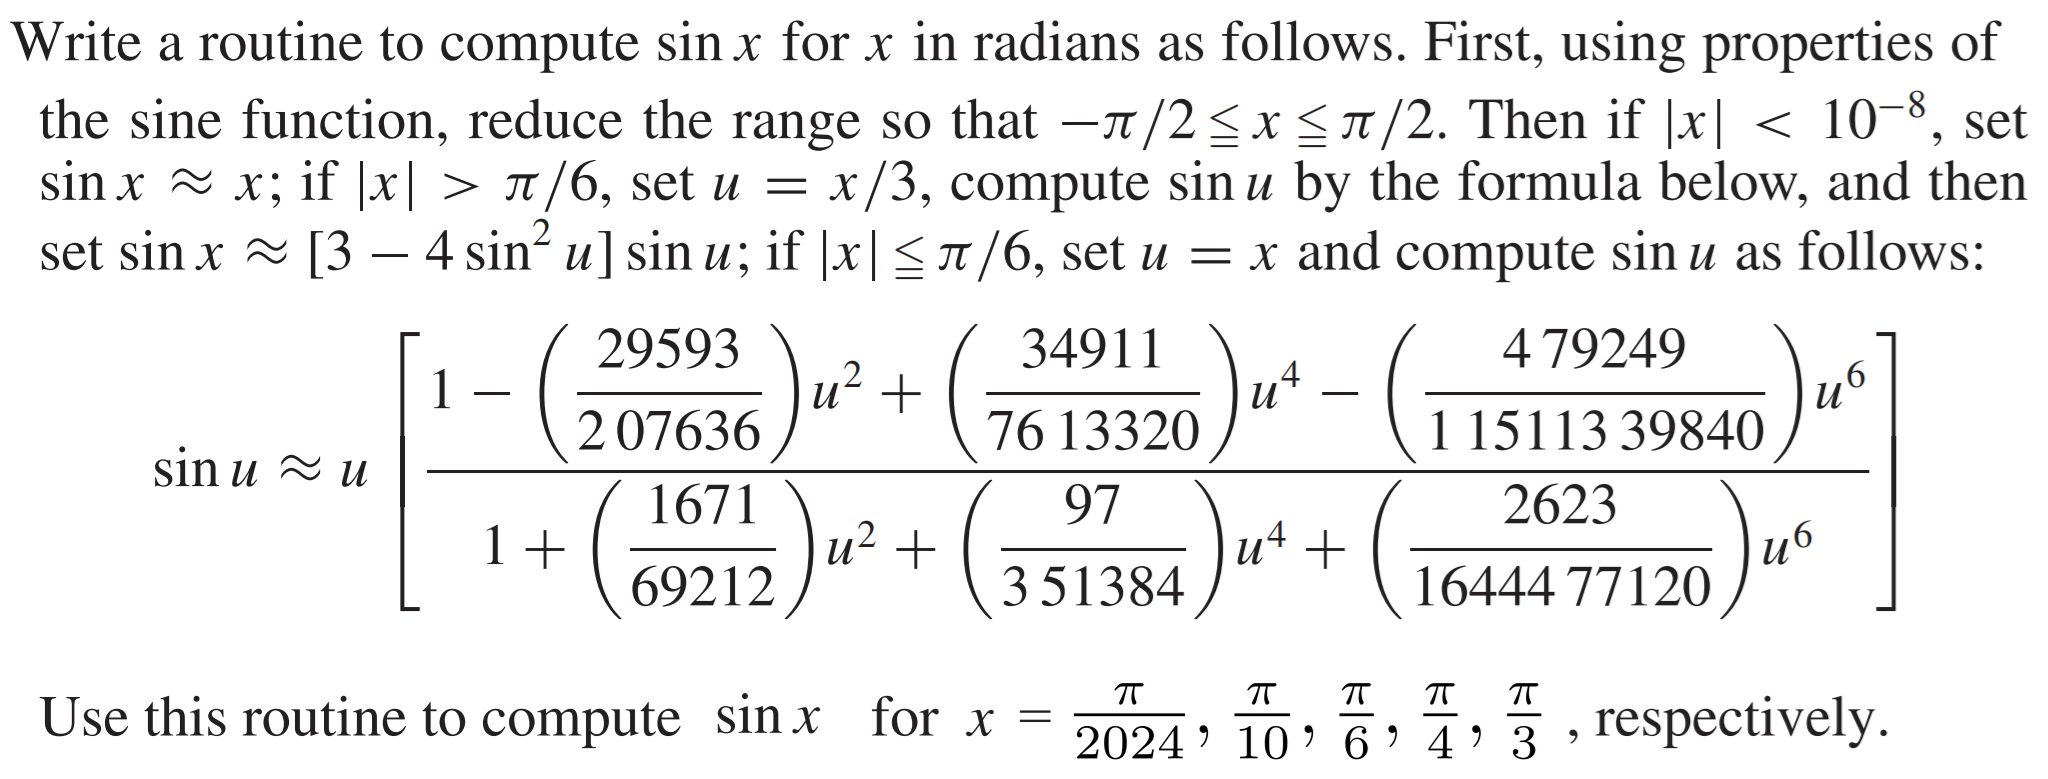
\includegraphics[width=5.40in,height=2.2in, angle=0]{image/lab01c}
  %\caption{\fontsize{9pt}{0pt} N=4 (Left), N=8 (Right)}
\end{figure}

\vspace{-0.2in}
Compare those results with results obtained by the Taylor formula, i.e., $\sin(x) \approx x- \frac{x^3}{3!} +  \frac{x^5}{5!} - \frac{x^7}{7!}$.
\end{itemize}

\clearpage

\section{数值结果(请尽量列表或作图)}
\begin{itemize}
  \item 问题1
\begin{table}[htb]
\begin{center}
\begin{tabular}{|c|c|c|} % 3列,每列居中对齐
\hline
$4^{-0}$ & 7.106781005859E-02 & 7.106781005859E-02 \\
\hline
$4^{-1}$ & 4.462718963623E-03 & 4.462862852961E-03 \\
\hline
$4^{-2}$ & 2.789497375488E-04 & 2.790123107843E-04 \\
\hline
$4^{-3}$ & 1.764297485352E-05 & 1.743859502312E-05 \\
\hline
$4^{-4}$ & 9.536743164062E-07 & 1.089913439500E-06 \\
\hline
$4^{-5}$ & 0.000000000000E+00 & 6.811959707420E-08 \\
\hline
$4^{-6}$ & 0.000000000000E+00 & 4.257474817138E-09 \\
\hline
$4^{-7}$ & 0.000000000000E+00 & 2.660921760711E-10 \\
\hline
$4^{-8}$ & 0.000000000000E+00 & 1.663076100444E-11 \\
\hline
$4^{-9}$ & 0.000000000000E+00 & 1.039422562778E-12 \\
\hline
$4^{-10}$ & 0.000000000000E+00 & 6.496391017361E-14 \\
\hline
$4^{-11}$ & 0.000000000000E+00 & 4.060244385850E-15 \\
\hline
\end{tabular}
\end{center}
\caption{题1计算结果}
\end{table}


虽然\(f(x)=g(x)\),但是\(f(x)\)与\(g(x)\)的计算结果在\(|x|\)较大时非常接近,但在\(x\)接近0时有所不同。

对\(f(x)\),当 \( x \) 接近 0 时,\( \sqrt{x^2 + 25} \) 接近 5。因此,\( f(x) = \sqrt{x^2 + 25} - 5 \) 的值也将接近 0。这种形式可能导致数值上的不稳定性,特别是在 \( x \) 非常小的情况下,因为从一个近似的常数中减去另一个近似相等的常数可能会导致显著的舍入误差。

对\(g(x)\),分子 \( x^2 \) 当 \( x \) 接近 0 时也接近 0,而分母 \( \sqrt{x^2 + 25} + 5 \) 在 \( x \) 接近 0 时接近 10。因此,\( g(x) \) 在 \( x \) 接近 0 时也将接近 0,但其形式导致计算更加稳定,因为分母较大且远离 0,避免了减法的不稳定性。


 \item  问题2~(用科学计数形式, 尾数至少保留9位小数)


 \begin{table}[htb]
 \begin{center}

\begin{tabular}{|c|c|}
\hline
      & Sum               \\ \hline
方法(a) & 1.2620010621E-11  \\ \hline
方法(b) & -6.8212102633E-11 \\ \hline
方法(c) & 4.6845403133E-11  \\ \hline
方法(d) & 0.0000000000E+00  \\ \hline
精确值  & 1.8563428950E-10  \\ \hline
\end{tabular}

\end{center}
\caption{题2计算结果}
\end{table}


从这些结果中可以看出,按照绝对值从大到小的顺序求和的方式(c)提供了比较精确的结果。

这是因为在此题中,计算结果非常靠近0,此时更小的数值在加到更大的数值时,其精确度的影响会减小,尤其是当小数值非常小比如接近浮点数的精度极限时。通过后加小数值,可以在某种程度上减少累积误差,这可能解释了为什么这种方式给出了精确的结果。

而其他方法中,由于较小数值的先行加和可能导致小数值的影响丢失,从而累积更大的误差。这个实验展示了不同求和顺序在数值稳定性上的影响,尤其是在处理涉及较大和较小数值的计算时。


 \item  问题3~(保留10位有效数字, $\pi \approx 3.14159 26535 897932$)
  \begin{table}[htb]
 \begin{center}
\begin{tabular}{|c|c|c|} % 4列,每列居中对齐
\hline
 $x$  & Special Routine for $\sin(x)$ & Taylor Approximation for $\sin(x)$  \\
\hline
  $\frac{\pi}{2024}$ & 1.55216966014E-03 & 1.55216966014E-03 \\
  \hline
  $\frac{\pi}{10}$ & 3.09016994375E-01 & 3.09016994293E-01 \\ \hline
  $\frac{\pi}{6}$ & 5.00000000000E-01 & 4.99999991869E-01 \\ \hline
  $\frac{\pi}{4}$ & 7.07106781187E-01 & 7.07106469575E-01 \\  \hline
  $\frac{\pi}{3}$ & 8.66025403784E-01 & 8.66021271656E-01 \\
\hline
\end{tabular}
\end{center}
\caption{题3计算结果}
\end{table}

 %$\frac{\pi}{2024}, \frac{\pi}{10}, \frac{\pi}{6}, \frac{\pi}{4}, \frac{\pi}{3}$

\end{itemize}


\section{算法分析}

在本次实验中,我们主要探讨了浮点数精度对数值计算结果的影响。我们通过不同的数学模型和近似方法,来分析和比较结果的精度和稳定性。

\begin{enumerate}
    \item \textbf{问题1} 使用单精度浮点数计算两个相同的函数的值,展示了在不同数量级的输入下,计算结果的精度如何受到影响。特别是当 \(x\) 接近 0 时,由于浮点数精度限制,从一个接近的常数中减去另一个近似相等的常数可能导致显著的舍入误差。
    \item \textbf{问题2} 探讨了不同的加法顺序对于最终求和结果的影响。这个实验通过四种不同的加法顺序展示了浮点数加法的不稳定性,尤其是在处理具有不同数量级的数值时。
    \item \textbf{问题3} 对比了特殊的正弦函数近似算法和泰勒级数展开式的结果,验证了算法的精度,并显示了不同算法在处理小角度时的高效性。
\end{enumerate}

\subsection*{关键发现}
\begin{itemize}
    \item \textbf{数值稳定性}:加法顺序显著影响求和结果的稳定性,其中按绝对值从小到大求和的方法在本实验中显示出最高的数值稳定性。
    \item \textbf{精度和效率}:在计算正弦函数时,使用特定的多项式近似比标准的泰勒级数方法提供了更高的计算效率和相似或更好的精度。
\end{itemize}

\section{实验小结}

本次实验不仅加深了我们对浮点数运算特性的理解,尤其是在精度和数值稳定性方面,还提供了对不同数值算法在实际应用中表现的深入洞察。通过对比不同算法的输出,我们可以更好地评估特定算法在特定情况下的适用性和效率。

\begin{itemize}
    \item \textbf{实用性评估}:对于需要高精度计算的应用,选择正确的算法和数学模型至关重要,尤其是在科学和工程领域。
    \item \textbf{算法选择}:实验结果强调了根据具体问题选择合适算法的重要性。例如,在处理小角度的三角函数计算时,使用针对性的多项式近似可以显著提高精度和计算速度。
\end{itemize}

通过这些实验,我们不仅提高了解决实际问题时的算法选择和设计能力,还增强了对计算机科学中浮点数运算限制的实际认识。这些经验对于未来在更广泛的科学研究和工程实践中具有重要价值。



\end{document}

